\subsection{PIMS Notification Module}
This module is responsible for sending email/SMS notifications to a patient. This email/text message could be a reminder to a patient about follow up visits to the doctor. \par 

\subsubsection{Scope}
The scope is shown in the use case diagram below: \par
\begin{figure}[H]
	\centerline{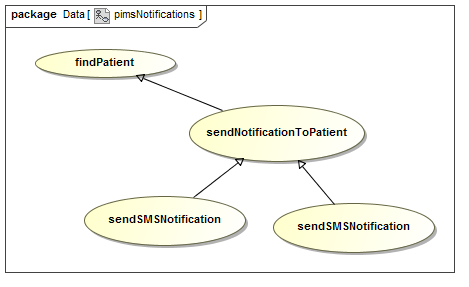
\includegraphics[width=0.75\linewidth]{./Graphics/pimsNotification/pimsNotifications}}
	\caption{The global scope for PIMS Notification Module}
\end{figure}

\subsubsection{Use cases}
\begin{description}
	\item{\textbf{findPatient -- [priority: nice-to-have]}}
	This use case is to cater for the retrieval of a patient ID/name form the database so as to obtain the contact details of the patient, if any.
	\begin{description}
		\item{\textbf{Service Contract}} The service contract for findPatient is shown below.
		\begin{figure}[H]
			\centerline{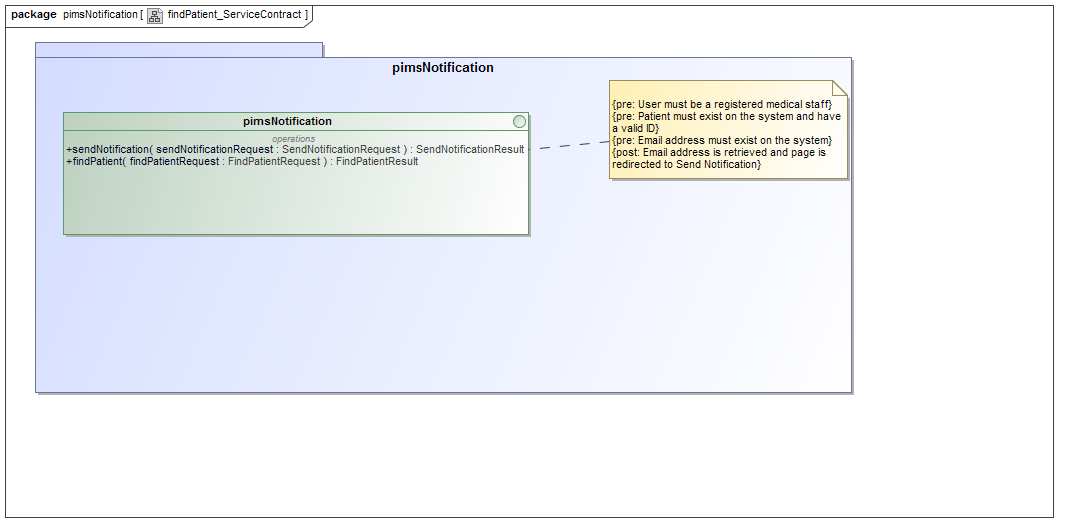
\includegraphics[width=0.7\linewidth]{./Graphics/pimsNotification/findPatient_ServiceContract}}
			\caption{Service contract for findPatient use case}
		\end{figure}
	\end{description}	
	
	\item{\textbf{sendNotification -- [priority: nice-to-have]}}
	This use case is to cater for the sending follow-up notification messages via SMS or email depending on whether or not the patient has an existing cellphone number or email.
	
		\begin{description}
		\item{\textbf{Service contract}} The service contract for sendNotification is shown below.
		\begin{figure}[H]
		\centerline{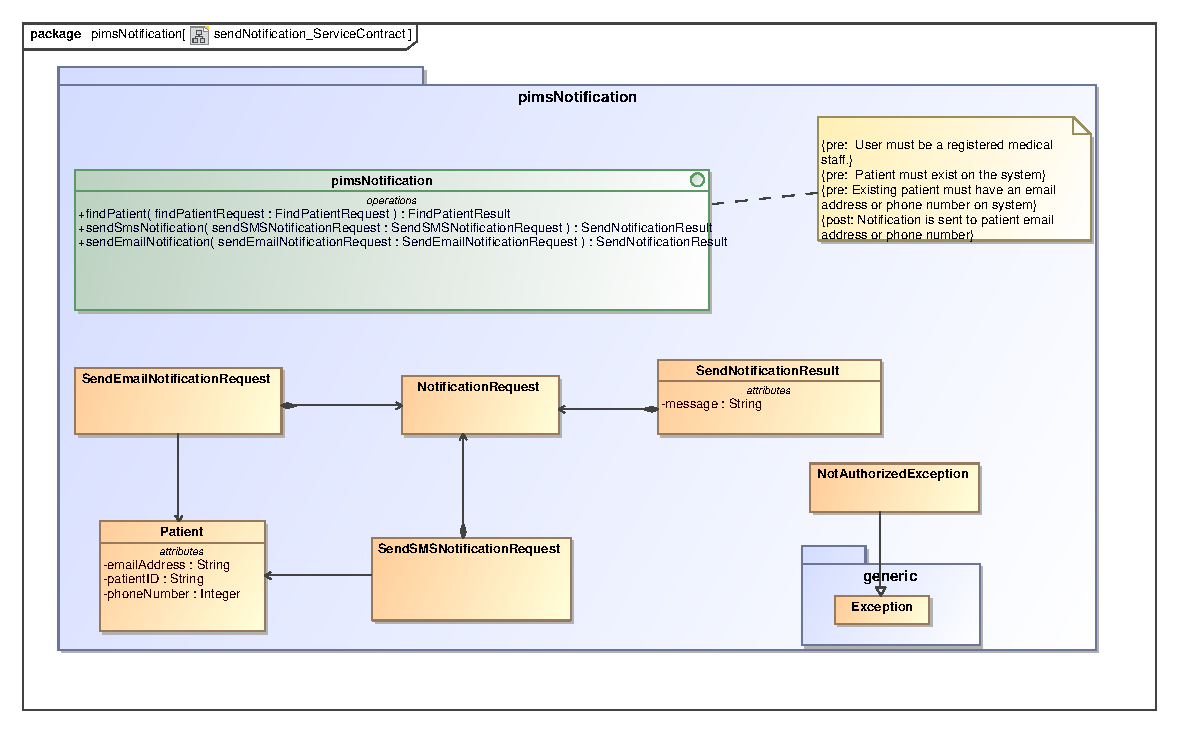
\includegraphics[width= 0.7\linewidth]{./Graphics/pimsNotification/sendNotification_ServiceContract}}
			\caption{Service contract for sendNotification }
		\end{figure}
	\end{description}
	\begin{description}
		\item{\textbf{Process specification}} The process specification for sendNotification is shown below.
		\begin{figure}[H]
		\centerline{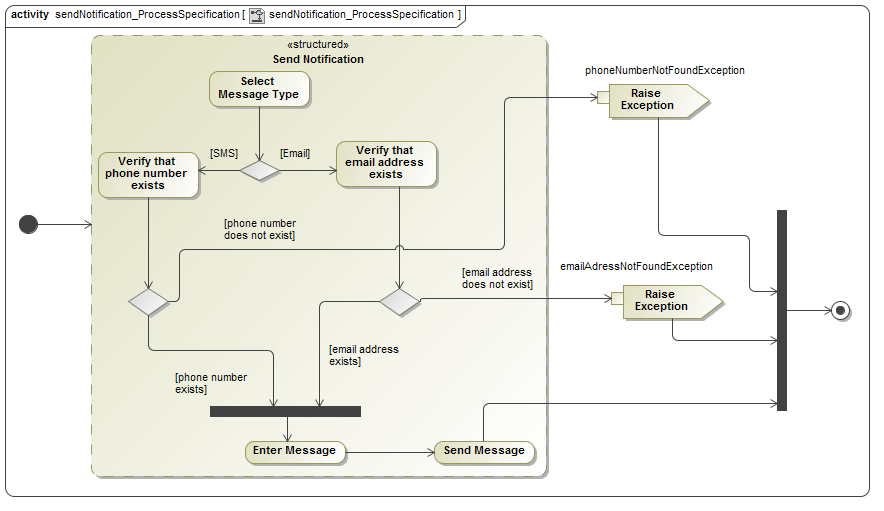
\includegraphics[width= 0.7\linewidth]{./Graphics/pimsNotification/sendNotification_ProcessSpecification}}
			\caption{Process specification for sendNotification }
		\end{figure}
	\end{description}		
	
\end{description}
